\maketitle
\tableofcontents
\newpage

\section{Zielsetzung}
In diesem Versuch geht es um Messung der Schwingungs- und Schwebungsdauer von gekoppelten Pendeln.
Untersucht werden gleich- und gegensinnige sowie gekoppelte Schwingungen.
\section{Theorie}
Ein einzelnes Fadenpendel, welches reibungsfrei aufgehängt wurde, mit einem Faden der Länge $\textit{l}$ und Masse $\textit{m}$,
schwingt für kleine Auslenkungen (sin $\phi \approx \phi$) mit der Schwingungsfrequenz
\begin{equation}
  \omega = \sqrt{\frac{g}{l}}
  \label{e1}
\end{equation}
Dies ist die Lösung der zugehörigen Schwingungsdifferentialgleichung mit g als Erdbeschleunigungskonstante. Mit \eqref{e1} und
\begin{equation*}
  \textit{T} = \frac{2\pi}{\omega}
\end{equation*}
ergibt sich als Formel für die gesuchte Schwingungsdauer
\begin{equation}
  \textit{T} = 2\pi \sqrt{\frac{l}{g}}
  \label{e2}
\end{equation}
Wenn man nun zwei dieser Fadenpendel durch eine Feder koppelt, ergeben sich zwei Differentialgleichungen:
\begin{equation}
  \begin{split}
    J \ \ddot{\Phi}_1 + D \ \Phi_{1} = D_{F} \ (\Phi_{2} - \Phi_{1}) \\
    J \ \ddot{\Phi}_2 + D \ \Phi_{2} = D_{F} \ (\Phi_{1} - \Phi_{2})
  \end{split}
\end{equation}
mit jeweils einem Term darin,
der den Drehwinkel des anderen Pendels enthält. Dies kommt durch die Kopplung mit der Feder. Je nach Auslenkungswinkel $\alpha_{1}$
und $\alpha_{2}$ der Fadenpendel ergeben sich verschiedene Schwingungsarten:
\\
\\
Für: $\alpha_{1} = \alpha_{2}$ ergibt sich eine gleichsinnige Schwingung. Bei dieser hat die Feder keine Auswirkung auf die
Schwingungen. Deshalb gilt für die Schwingungsfrequenz $\omega_{+}$ \eqref{e1} und für die Schwingungsdauer $\textit{T}_{+}$
\eqref{e2}.
\\
\\
Wenn $\alpha_{1} = -\alpha_{2}$ ist, nennt man dies eine gegensinnige Schwingung. Für diesen Fall greift die Feder in das Schwingverhalten
der Pendel ein. Deshalb werden \eqref{e1} und \eqref{e2} erweitert um jeweils einen Term mit der Kopplungskonstante $\textit{K}$
der Feder
\begin{equation}
  \omega_{-} = \sqrt{\frac{g}{l} + \frac{2 K}{l}}
  \label{e3}
\end{equation}
\begin{equation}
  \textit{T}_{-} = 2\pi  \sqrt{\frac{l}{g + 2 \textit{K}}}
  \label{e4}
\end{equation}
\\
\\
Für: $\alpha_{1} = 0, \alpha_{2} \neq 0$ ergibt sich eine gekoppelte Schwingung. Diese zeichnet sich dadurch aus, dass die beiden
Pendel die kinetische Energie auf das andere Pendel übertragen und dann erneut erhalten. Hier tritt die sogenannte Schwebung auf.
Dieser Begriff beschreibt die Zeit zwischen zwei Stillständen eines Pendels. Die Dauer dieses Zustandes berechnet sich nach
\begin{equation}
  \textit{T}_{S} = \frac{\textit{T}_{-} \cdot \textit{T}_{+}}{\textit{T}_{+} - \textit{T}_{-}}
  \ \ \text{und} \ \ \omega_{S} = \omega_{+} - \, \omega_{-}
  \label{e5}
\end{equation}
mit $\textit{T}_{-}$ aus der gegen- und $\textit{T}_{+}$ aus der gleichsinnigen Schwingung. Die Kopplungskonstante \textit{K}
der Feder zwischen den beiden Pendeln definiert sich nach
\begin{equation}
  \textit{K} = \frac{\textit{T}_{+}^{2} - \textit{T}_{-}^{2}}{\textit{T}_{+}^{2} + \textit{T}_{-}^{2}} =
  \frac{\omega_{-}^{2} - \omega_{+}^{2}}{\omega_{-}^{2} + \omega_{+}^{2}}
  \label{e6}
\end{equation}
\section{Durchführung}
Die Pendel sind zwei Stabpendel, die verschieboverlinee Massen besitzen, um verschiedene Pendellängen zu realisieren. Die
Aufhängung besteht aus einer reibungsarmen Spitzenlagerung, die eine reibungsfreie Schwingung gewährleistet.
\begin{figure}[h]
  \centering
  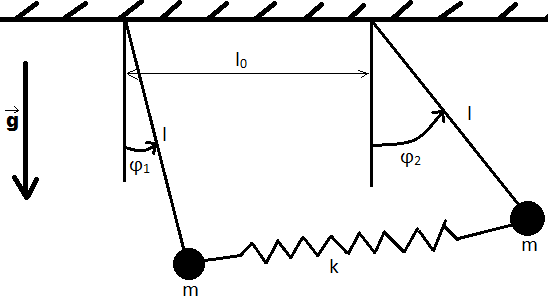
\includegraphics{gekoppelte_pendel2.png}
  \caption{Darstellung eines gekoppelten Pendels mit Öffnungswinkeln $\phi$ statt $\alpha$.}
  \label{fig:skizze1}
\end{figure}
Alle Schwingungsdauern werden für fünf Schwingungen und für eine Pendellänge von $\SI{60.0(3)}{\centi\metre}$ bestimmt. Zuerst messen wir die Schwingungsdauern $\textit{T}_{1}$
und $\textit{T}_{2}$ der einzelnen Pendel nach und vergleichen, ob sie im Rahmen der Messgenauigkeit übereinstimmen. Um eventuellen
statistischen Fehlern vorzubeugen, führen wir die Messung neunmal aus. Danach verbinden wir die beiden Pendel über die Kopplungsfeder und führen eine gleich-
und eine gegensinnige Schwingung durch , wobei wir $\textit{T}_{+}$ und $\textit{T}_{-}$ experimentell bestimmen. Im
Anschluss ermitteln wir die Schwebungsdauer $\textit{T}_{S}$ und die Schwingungsdauer $\textit{T}$. Zum Schluss wiederholen wir
alle Messungen für eine Pendellänge von $\SI{75.0(3)}{\centi\metre}$.
\section{Fehlerrechnung}
Für die Fehlerrechnung gibt:
\begin{equation}
  \overline{T} = \frac{1}{n} \sum_{i=1}^{n} T_{i}
\end{equation}
den Mittelwert, sowie:
\begin{equation}
  \sigma_{\overline{T}} = \sqrt{\frac{1}{n(n-1)} \sum_{i=1}^{n}(\overline{T}-T_i)^2}
\end{equation}
den Fehler des Mittelwertes.
In Fällen, in denen zwei fehlerbehaftete Größen in einer Gleichung zur Bestimmung einer anderen Größe Verwendung finden, berechnt sich der Gesamtfehler
nach der Gaußschen Fehlerfortpflanzung zu:
\begin{equation}
    \symup \Delta f(x_1, x_2, ..., x_n) = \sqrt{\left(\frac{\symup df}{\symup dx_1} \symup \Delta
    x_1 \right)^2 +    \left(\frac{\symup df}{\symup dx_2} \symup \Delta
    x_2 \right)^2 + ... + \left(\frac{\symup df}{\symup dx_n} \symup \Delta x_n \right)^2} \ .
\end{equation}
\section{Auswertung}
\subsection{Berechnung der Schwingungsdauern der entkoppelten Pendel}
Es wurden jeweils 10 Messungen für jeweils 5 Schwingungen durchgeführt.
Aus den Messwerten folgen die in der Tabelle dargestellten Schwingungdauern für die jeweils entkoppelten Pendel.
\begin{table}
  \centering
  \caption{Entkoppelte Pendel für 5 Schwingungen}
  \label{tab:data1}
  \begin{tabular}{S S S S}
    \toprule
    \multicolumn {2}{c}{$l = \SI{60.0(3)}{\centi\metre}$} & \multicolumn {2}{c}{$l = \SI{75.0(3)}{\centi\metre}$}\\
    {$T_1$/\si{\second}} & {$T_2$/\si{\second}} & {$T_1$/\si{\second}} & {$T_2$/\si{\second}} \\
    \midrule
    7.49 & 7.33 & 8.49 & 8.13 \\
    7.36 & 7.30 & 8.46 & 8.01 \\
    7.30 & 7.00 & 8.33 & 8.44 \\
    7.61 & 7.30 & 8.20 & 8.46 \\
    7.32 & 7.58 & 8.23 & 8.16 \\
    7.26 & 7.27 & 8.15 & 8.20 \\
    7.60 & 7.46 & 8.20 & 8.15 \\
    7.81 & 7.50 & 8.40 & 8.52 \\
    7.27 & 7.35 & 8.01 & 8.16 \\
    7.52 & 7.55 & 7.78 & 8.67 \\
    \bottomrule
  \end{tabular}
\end{table}
\\
Es ergeben sich folgende Werte für $\SI{60.0(3)}{\centi\metre}$:
\begin{equation*}
\begin{split}
  \overline{T_1} = \SI{1.49(1)}{\second} \\
  \overline{T_2} = \SI{1.47(1)}{\second}
\end{split}
\end{equation*}
\\
Und für $\SI{75.0(3)}{\centi\metre}$:
\begin{equation*}
\begin{split}
  \overline{T_1} = \SI{1.65(1)}{\second}\\
  \overline{T_2} = \SI{1.66(1)}{\second}
\end{split}
\end{equation*}
\\
Die Werte der Schwingungsdauern liegen also bei beiden längen gegenseitig im Bereich der Messabweichung.
\subsection{Berechnung der Schwingfrequenzen bei gleich- und gegensinniger Schwingung}
Es werden weiterhin die in 4.1 eingeführten Formeln zur Fehlerrechnung genutz.
Aus den Messwerten folgen die in der Tabelle dargestellten Schwingungdauern für die jeweils entkoppelten Pendel.
\begin{table}[h]
  \centering
  \caption{Gegen- und gleichsinnige Schwingung für 5 Schwingungen}
  \label{tab:data2}
  \begin{tabular}{S S S S}
    \toprule
    \multicolumn {2}{c}{$\SI{60.0(3)}{\centi\metre}$} & \multicolumn {2}{c}{$\SI{75.0(3)}{\centi\metre}$}\\
    {$T_+$/\si{\second}} & {$T_-$/\si{\second}} & {$T_+$/\si{\second}} & {$T_-$/\si{\second}} \\
    \midrule
    7.70 & 7.04 & 8.75 & 7.84 \\
    7.47 & 7.18 & 8.90 & 7.92 \\
    7.26 & 6.95 & 8.66 & 8.03 \\
    7.47 & 7.21 & 8.60 & 7.69 \\
    7.49 & 6.96 & 8.42 & 7.81 \\
    7.32 & 7.03 & 8.46 & 7.63 \\
    7.09 & 7.32 & 8.53 & 7.72 \\
    7.43 & 7.04 & 8.33 & 7.87 \\
    7.55 & 7.03 & 8.30 & 7.44 \\
    7.16 & 7.30 & 8.49 & 7.61 \\
    \bottomrule
  \end{tabular}
\end{table}
\\
Es ergeben sich folgende Werte für $\SI{60.0(3)}{\centi\metre}$:
\begin{equation*}
\begin{split}
  \overline{T_+} = \SI{1.48(1)}{\second}\\
  \overline{T_-} = \SI{1.42(1)}{\second}
\end{split}
\end{equation*}
\\
Und für $\SI{75.0(3)}{\centi\metre}$:
\begin{equation*}
\begin{split}
  \overline{T_+} = \SI{1.71(1)}{\second}\\
  \overline{T_-} = \SI{1.55(1)}{\second}
\end{split}
\end{equation*}
\\
Nach Gauß'scher Fehlerfortpflanzung und mit \eqref{e1} sowie \eqref{e3} folgt für die Frequenzen bei $\SI{60.0(3)}{\centi\metre}$:
\begin{equation*}
\begin{split}
  \omega_+ = \SI{4.249(34)}{\per\second}\\
  \omega_- = \SI{4.421(27)}{\per\second}
\end{split}
\end{equation*}
\\
Und für $\SI{75.0(3)}{\centi\metre}$:
\begin{equation*}
\begin{split}
  \omega_+ = \SI{3.677(26)}{\per\second}\\
  \omega_- = \SI{4.051(28)}{\per\second}
\end{split}
\end{equation*}
\\
Für die Kopplungskonstante ergibt sich nach \eqref{e6} daher bei $\SI{60.0(3)}{\centi\metre}$:
\begin{equation*}
  K = \num{0.040(10)}
\end{equation*}
\\
Und für $\SI{75.0(3)}{\centi\metre}$:
\begin{equation*}
  K = \num{0.096(10)}
\end{equation*}
\\
\subsection{Vergleich zwischen gemessenen und errechneten Werten}
Für $T_+ \text{ und } \omega_+$ folgt aus \eqref{e1} und \eqref{e2} bei $l = \SI{60.0(3)}{\centi\metre}$:
\begin{equation*}
  \begin{split}
  T_+ = \SI{1.554(4)}{\second} \\
  \omega_+ = \SI{4.043(10)}{\per\second}
  \end{split}
\end{equation*}
und für $l = \SI{75.0(3)}{\centi\metre}$:
\begin{equation*}
  \begin{split}
      T_+ = \SI{1.738(3)}{\second} \\
      \omega_+ = \SI{3.616(7)}{\per\second}
  \end{split}
\end{equation*}
Beim Vergleich dieser Werte mit den gemessenen Werten zeigen sich Abweichungen, die außerhalb der Ungenauigkeiten liegen.
\\
Für $T_- \text{ und } \omega_-$ folgt aus \eqref{e3} und \eqref{e4} bei $l = \SI{60.0(3)}{\centi\metre}$:
\begin{equation*}
  \begin{split}
  T_- = \SI{1.548(4)}{\second} \\
  \omega_- = \SI{4.059(11)}{\per\second}
  \end{split}
\end{equation*}
und für $l = \SI{75.0(3)}{\centi\metre}$ bei gleicher Ungenauigkeit:
\begin{equation*}
  \begin{split}
      T_- = \SI{1.721(4)}{\second} \\
      \omega_- = \SI{3.651(8)}{\per\second}
  \end{split}
\end{equation*}
Beim Vergleich dieser Werte mit den gemessenen Werten zeigen sich Abweichungen, die außerhalb der Ungenauigkeiten liegen.
Nach \eqref{e5} ergibt sich die Schwingungsdauer sowie -frequenzen bei der gekoppelten Schwingung mit $\SI{60.0(3)}{\centi\metre}$ zu:
\begin{equation*}
  \begin{split}
  T_s = \SI{36(9)}{\second} \\
  \omega_s = \SI{0.170(40)}{\per\second}
  \end{split}
\end{equation*}
\\
Und für $\SI{75.0(3)}{\centi\metre}$:
\begin{equation*}
  \begin{split}
  T_s = \SI{16.8(17)}{\second} \\
  \omega_s = \SI{0.370(40)}{\per\second}
\end{split}
\end{equation*}
Die Fehler ergeben sich jeweils durch Gaußsche Fehlerfortpflanzung aus den Fehlerbehafteten Größen $T_+$ und $T_-$.
\\
\begin{table}[b]
  \centering
  \caption{Schwebungsdauer bei Messung einer Schwebung für eine Schwebung}
  \label{tab:data3}
  \begin{tabular}{c c}
    \toprule
    $T_{s}/\si{\second} \text{ für } l=\SI{60.0(3)}{\centi\metre}$ & $T_{s}/\si{\second} \text{ für } l=\SI{75.0(3)}{\centi\metre}$ \\
    \midrule
    29.41 & 36.46 \\
    28.87 & 37.03 \\
    29.07 & 33.87 \\
    31.67 & 34.06 \\
    28.63 & 31.01 \\
    28.46 & 38.27 \\
    31.73 & 36.55 \\
    33.60 & 32.32 \\
    28.96 & 33.10 \\
    30.80 & 38.47 \\
    \bottomrule
  \end{tabular}
\end{table}
\\
\begin{table}[b]
  \centering
  \caption{Schwebungsdauer bei Messung von fünf Schwebungen für 5 Schwebungen}
  \label{tab:data4}
  \begin{tabular}{c c}
    \toprule
  $T_{s}/\si{\second} \text{ für } l=\SI{60.0(3)}{\centi\metre}$ & $T_{s}/\si{\second} \text{ für } l=\SI{75.0(3)}{\centi\metre}$ \\
    \midrule
    135.52 & 185.12 \\
    138.58 & 208.84 \\
    150.44 & 191.00 \\
    157.96 & 206.87 \\
    124.87 & 209.01 \\
    138.24 & 214.86 \\
    164.76 & 204.83 \\
    \bottomrule
  \end{tabular}
\end{table}
Aus den gemessenen Werten (siehe Tabelle 3 und 4) folgt für $\overline{T_s}$ und $\overline{\omega_s}$, gemessen bei $\SI{60.0(3)}{\centi\metre}$:
\begin{equation*}
\begin{split}
 \text{Einzelmessung: }\overline{T_{s}} = \SI{30.1(5)}{\second}; \ \ \ \overline{\omega_s}= \SI{0.209(4)}{\per\second}\\
 \text{Fünffachmessung: }\overline{T_{s}} = \SI{28.9(11)}{\second}; \ \ \ \overline{\omega_s} = \SI{0.218(8)}{\per\second}
\end{split}
\end{equation*}
\\ und bei $\SI{75.0(3)}{\centi\metre}$
\begin{equation*}
\begin{split}
 \text{Einzelmessung: }\overline{T_{s}} = \SI{35.1(8)}{\second}; \ \ \ \overline{\omega_s} = \SI{0.217(8)}{\per\second}\\
 \text{Fünffachmessung: }\overline{T_{s}} = \SI{40.6(8)}{\second}; \ \ \ \overline{\omega_s} = \SI{0.158(4)}{\per\second}
\end{split}
\end{equation*}
Für die Messung bei $\SI{60.0(3)}{\centi\metre}$ liegen die gemessene Werte für $T_s$ und $ \omega_s = 2\pi/T_s$ im Rahmen der zu erwartenden Abweichung für den berechneten Wert,
bei $\SI{75.0(3)}{\centi\metre}$ ist dies nicht der Fall.
\section{Diskussion}
Generell zeigen sich Abweichungen zwischen Messwerten und berechneten Werten, die sich vielfach nicht im Bereich der Messungenauigkeit bewegen.
Besonders bei der zweiten Schwebungsmessung ist dies nicht der Fall. Gründe finden sich hier in der Dämpfung des Pendels, durch die sich mit fortschreitender Zeit eine
Verschiebung von Schwebung zu gleichphasiger Schwingung sowie generelle Fehler in der Zeitmessung ergeben. Auch die Feder kann nicht mehr als vollständig elastisch
angenommen werden. Definitiv einen statistischen Fehler stellt das stoppen der Zeiten mit einer Stopuhr dar. Dieser fließt zwar durch die Messmethoden nur gemindert ein,
beeinflusst das Ergebnis aber dennoch. Auch eine perfekt 2-Dimensionale Bewegung des Pendels lässt sich nicht sicherstellen, da der Stab elastisch ist.
Durch diese Fehler lassen sich auch die Unterschiede der Kopplungskonstante der beiden Messreihen erklären. Diese liegen ebenfalls nicht mehr im Ramen der Messungenauigkeit.
\\
Zusammenfassend zeigt sich nur eine geringe Aussagekraft des Versuchs. In der vorgefundenen Konfiguration des Aufbaus lassen sich keine ausreichend präzisen Werte bestimmen.
Die durch die Zeitmessung erhaltenen Fehler lassen sich durch mehr Messungen verringern. Um die Dämpfung durch Luftreibung und Auflagefläche zu verringern ist ein deutlich höherer
Aufwand zu betreiben. Die Abweichung der Bewegung eine dritte Raumrichtung ließe sich durch einen weniger elastischen Stab minimieren.

\newpage
\nocite{*}
\printbibliography
